% ============================================================
% Defense slides - A Digital Twin for EV Battery Monitoring
% Chao Song - Politecnico di Torino - M.Sc. Computer Engineering
%
% Compile:  pdflatex slides.tex  (run twice)
%           latexmk -pdf slides.tex
%
% Font: TeX Gyre Adventor (sans) - the TeX Live stand-in for
% Century Gothic. To use the original font: place Century
% Gothic .ttf files in presentation/fonts/, switch engine to
% lualatex, and replace the tgadventor block with fontspec.
%
% TODO before the defense: set \defensedate below.
% ============================================================
\documentclass[11pt,aspectratio=169]{beamer}

% ---------------- font: Century Gothic stand-in ----------------
\usepackage[T1]{fontenc}
\usepackage{lmodern}          % math + fallback text
\usepackage{tgadventor}       % TeX Gyre Adventor
\renewcommand{\sfdefault}{qag}% all beamer text in Adventor
\usepackage{microtype}

% ---------------- packages ----------------
\usepackage{booktabs}
\usepackage{array}
\usepackage{makecell}

% ---------------- colors ----------------
\definecolor{politoblue}{RGB}{0,92,171}   % PoliTo blue
\definecolor{ink}{RGB}{11,11,11}
\definecolor{alertred}{RGB}{208,59,59}
\setbeamercolor{alerted text}{fg=alertred}
\setbeamercolor{block title}{bg=politoblue,fg=white}
\definecolor{blockbody}{RGB}{236,242,249}
\setbeamercolor{block body}{bg=blockbody}

% ---------------- theme ----------------
\usetheme{Madrid}
\usecolortheme[named=politoblue]{structure}
\setbeamertemplate{navigation symbols}{}
\setbeamertemplate{itemize item}{\textbullet}
\setbeamertemplate{itemize subitem}{--}
\setbeamertemplate{blocks}[rounded][shadow=false]
\graphicspath{{../images/}{../images/logo/}{figures/}}

% ---------------- metadata ----------------
\newcommand{\defensedate}{DD Month 2026}  % TODO: set real date
\title[A Digital Twin for EV Battery Monitoring]{A Digital Twin for EV Battery Monitoring}
\subtitle{Lightweight SoH Estimation on an Automotive Microcontroller}
\author[Chao Song]{Chao Song}
\institute[PoliTo --- M.Sc. Computer Engineering]{Politecnico di Torino --- M.Sc. in Computer Engineering\\[0.3em]
Supervisors: Prof.\ Sara Vinco \ \ $\cdot$ \ \ Dr.\ Khaled Sidahmed Sidahmed Alamin}
\date{\defensedate}
\titlegraphic{
\includegraphics[height=1.4cm]{logoPoliTo_symbol_only.pdf}}

\begin{document}

% ================================================================
%  1. Title
% ================================================================
\begin{frame}[plain]
  \titlepage
\end{frame}
\note{Good morning. My thesis brings SoH estimation for EV batteries onto the
vehicle's own microcontroller. In the next 15 minutes I will show why that is
hard, what I built, and how it performed on real hardware.}

% ================================================================
%  Motivation
% ================================================================
\section{Motivation}

% ---- 2. Motivation & SoH ----
\begin{frame}{Motivation \& SoH}
  \begin{columns}[T]
    \begin{column}{0.42\textwidth}
      \begin{itemize}
        \item Global EV sales: 3M (2020) $\rightarrow$ 16.6M (2024), CAGR $\approx$ 53\% {\footnotesize(IEA)}
        \item The battery is the most critical --- and expensive --- component
        \item The BMS must track two states:
        \begin{itemize}
          \item \textbf{SoC} --- minutes to hours
          \item \textbf{SoH} --- months to years
        \end{itemize}
        \item $SoH = \frac{C_{current}}{C_{initial}} \times 100\%$; below 70--80\% = end of life
      \end{itemize}
    \end{column}
    \begin{column}{0.55\textwidth}
      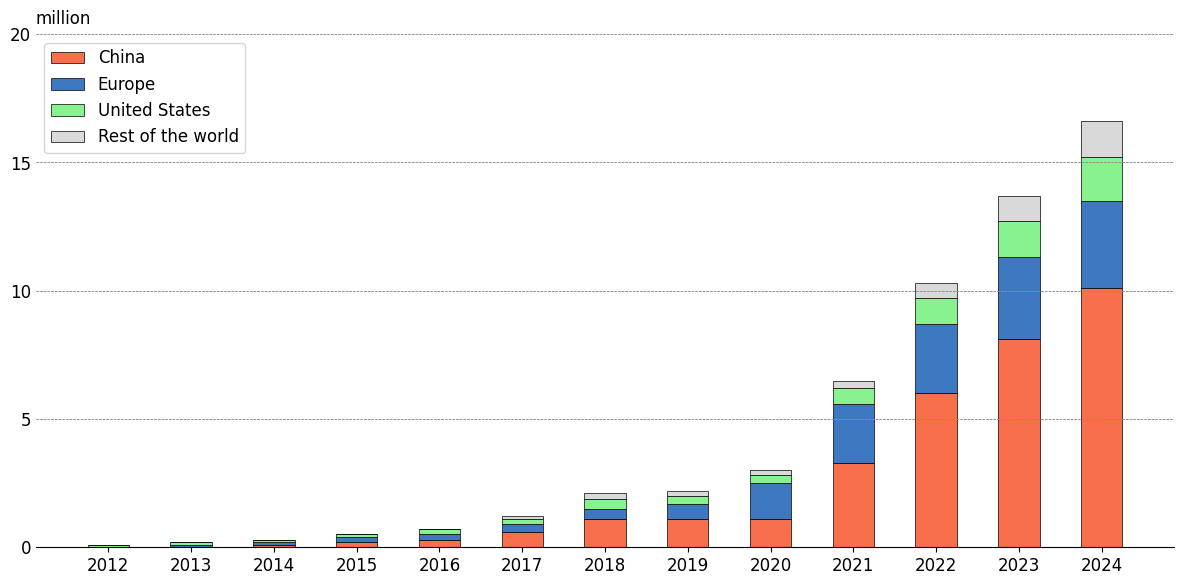
\includegraphics[width=\textwidth]{ch1_EV_sales.png}
    \end{column}
  \end{columns}
  \begin{alertblock}{The problem this thesis attacks}
    SoH has \textbf{no sensor} --- it must be \textbf{inferred}.
    Aging is nonlinear, multi-factor coupled, and path-dependent.
  \end{alertblock}
\end{frame}
\note{Every one of these vehicles carries a battery pack whose health determines
safety, range, and cost. The BMS must know that health in real time. SoH, the
fraction of original capacity left, has no sensor; it must be inferred, and aging
is nonlinear, coupled, and path-dependent.}

% ================================================================
%  Problem
% ================================================================
\section{Problem}

% ---- 3. Four barriers ----
\begin{frame}{Problem: four barriers to an on-board estimator}
  \begin{enumerate}
    \item \textbf{Model-based hits a wall} --- P2D too heavy for an MCU;
          ECM + Kalman drifts as the battery ages
    \item \textbf{Data-driven stops at simulation} --- ML is accurate (MAE $<2\%$)
          but almost never leaves the Python notebook
    \item \textbf{Cloud vs.\ edge: neither is free} --- cloud: latency, bandwidth,
          privacy; edge MCU: $\sim\!10^5\times$ fewer resources than the training server
    \item \textbf{SoC--SoH coupling} --- SoC needs the \emph{current} SoH;
          a stale SoH $\Rightarrow$ systematically biased SoC
  \end{enumerate}
  \vspace{0.4em}
  \begin{block}{}
    Each layer exposes the next. \textbf{SoH is where everything starts.}
  \end{block}
\end{frame}
\note{The gap between the literature and a working on-board estimator is four
layers deep. Physics models are too heavy or drift. ML models never leave the
server. The cloud cannot be trusted with a safety-critical loop, and the edge has
almost no resources. And even if you solve all that, SoC estimation needs the
current SoH, so SoH is where everything starts.}

% ---- 4. Digital Twin vision & the gap ----
\begin{frame}{A Digital Twin vision --- and the gap it exposes}
  \begin{columns}[T]
    \begin{column}{0.52\textwidth}
      \small
      \begin{itemize}
        \item Dual-model architecture (Alamin):
        \begin{itemize}
          \item \textbf{SoH model}: deployed once, robust for the long term
          \item \textbf{SoC model}: refreshed over the air as SoH drifts
        \end{itemize}
        \item This thesis: \textbf{build \& deploy the SoH foundation}, design the OTA channel
        \item Baseline (Sammartino et al.): BiLSTM on SPC58 --- but a \textbf{fixed
              20-sample window}, full-charge start
        \item Fixed tensor shape $\Rightarrow$ a new window length = retraining
              (5 lengths would need 5 models)
      \end{itemize}
    \end{column}
    \begin{column}{0.42\textwidth}
      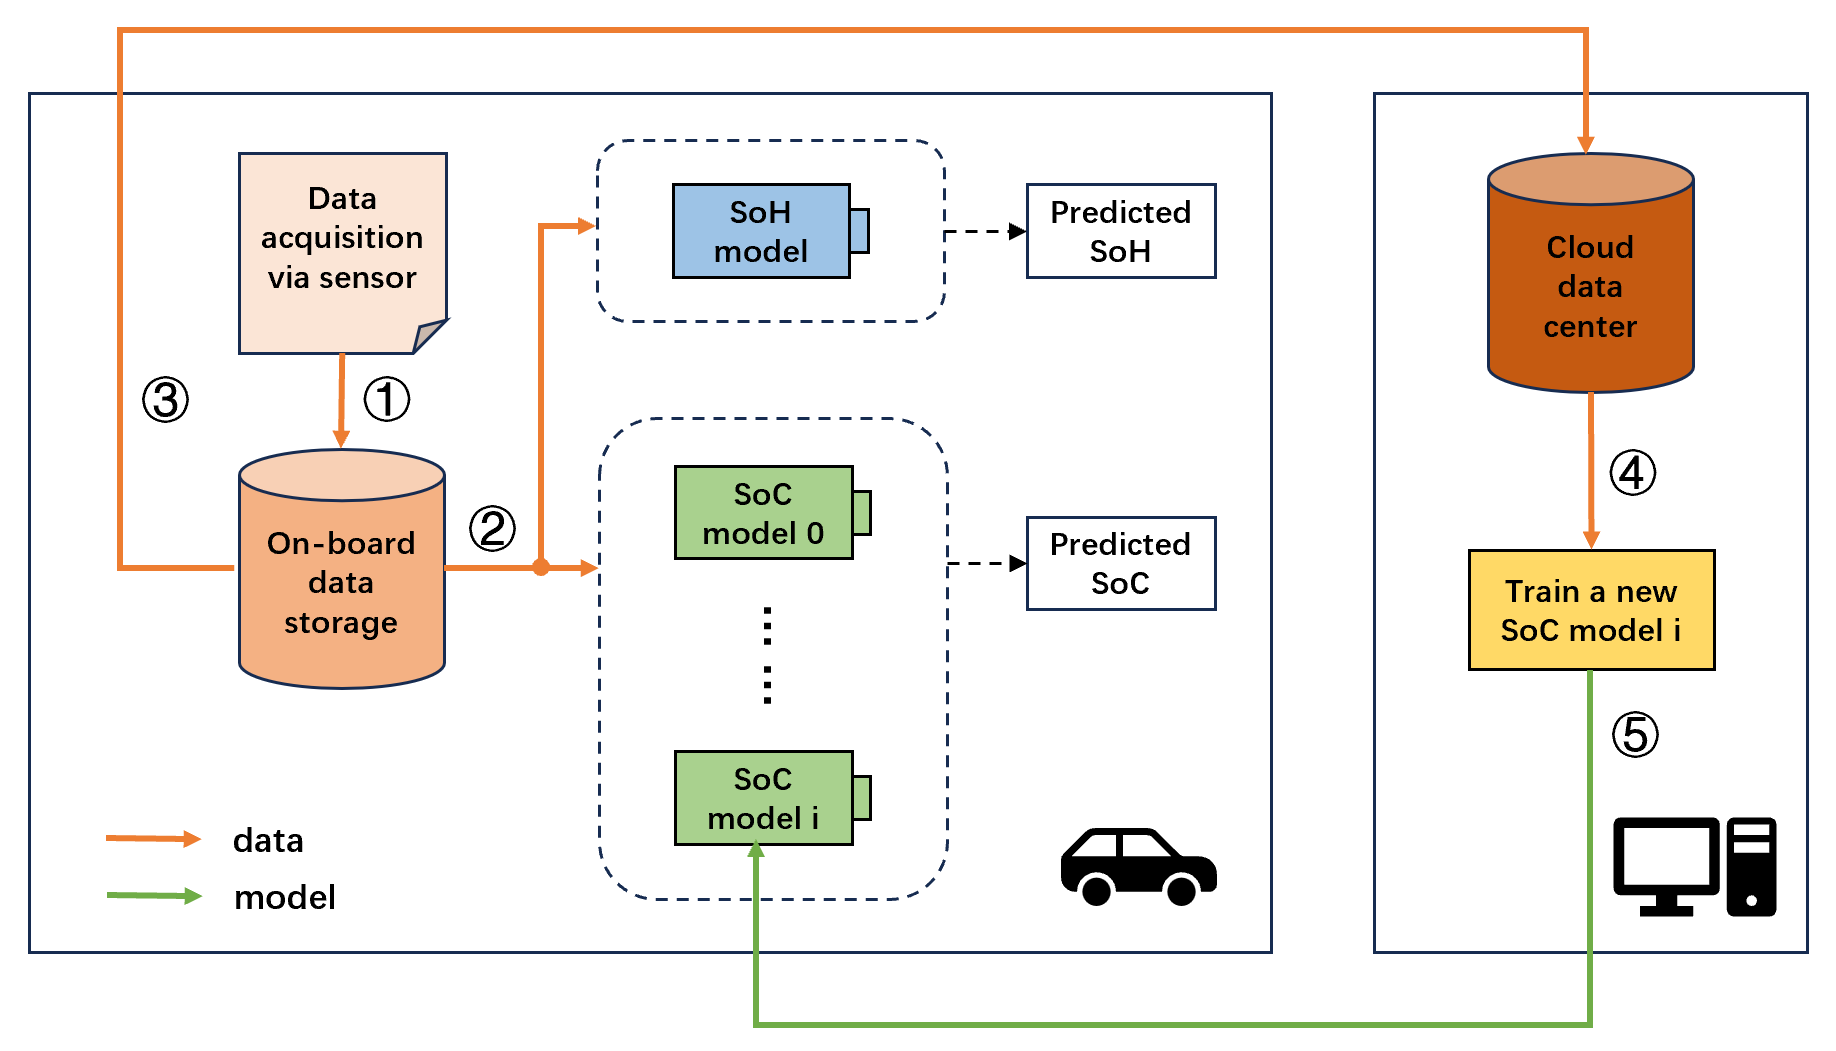
\includegraphics[width=\textwidth]{ch3_project_architecture.png}
      \vspace{0.3em}
      \begin{block}{Research question}
        Can one model be trained \emph{once} and stay accurate on \emph{any} input window length?
      \end{block}
    \end{column}
  \end{columns}
\end{frame}
\note{In this architecture SoH is the foundation: the SoC model consumes the SoH
estimate, so SoH must be right first. The baseline is one of the very few fully
deployed works, but it fixes the input window at 20 samples. In the field, trips
vary in length and sampling rates change across hardware generations. A fixed-shape
LSTM cannot adapt without retraining.}

% ================================================================
%  Contributions
% ================================================================
\section{Contributions}

% ---- 5. Aims & contributions ----
\begin{frame}{Aims \& contributions}
  \begin{enumerate}
    \item \textbf{Multi-length segmentation + 10-D feature extraction}
          $\rightarrow$ one model, any window length
    \item \textbf{LightGBM compiled to C}, deployed and validated on the
          SPC58EC80E5 automotive MCU
          \begin{itemize}
            \item matches BiLSTM accuracy --- 11--30$\times$ faster
          \end{itemize}
    \item \textbf{OTA update architecture design}
          (8-step lifecycle, A/B partitions, security)
  \end{enumerate}
\end{frame}
\note{I close the gap with three pieces of work. First, a training strategy that
makes window length irrelevant. Second, a tree-based model compiled to C and
running on automotive silicon. Third, the OTA design that keeps the companion SoC
model current over the battery's life.}

% ================================================================
%  Approach
% ================================================================
\section{Approach}

% ---- 6. Method overview ----
\begin{frame}{Method overview: one pipeline, five stages}
  \begin{center}
    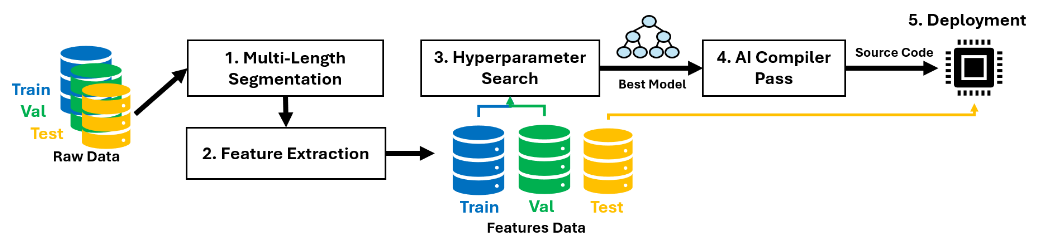
\includegraphics[width=0.9\textwidth]{ch3_ml_workflow.png}
  \end{center}
  \vspace{0.3em}
  {\small 1.\ data \& multi-length segmentation \quad 2.\ feature extraction \quad
  3.\ LightGBM + Bayesian HP search \quad 4.\ EDEN $\rightarrow$ C \quad
  5.\ MCU deployment \& verification}
\end{frame}
\note{The whole system is one pipeline of five stages. I will spend time on the two
design decisions that carry the thesis --- segmentation and feature extraction ---
then show how the model reaches the MCU.}

% ---- 7. Multi-length segmentation ----
\begin{frame}{Multi-length segmentation}
  \begin{columns}[T]
    \begin{column}{0.58\textwidth}
      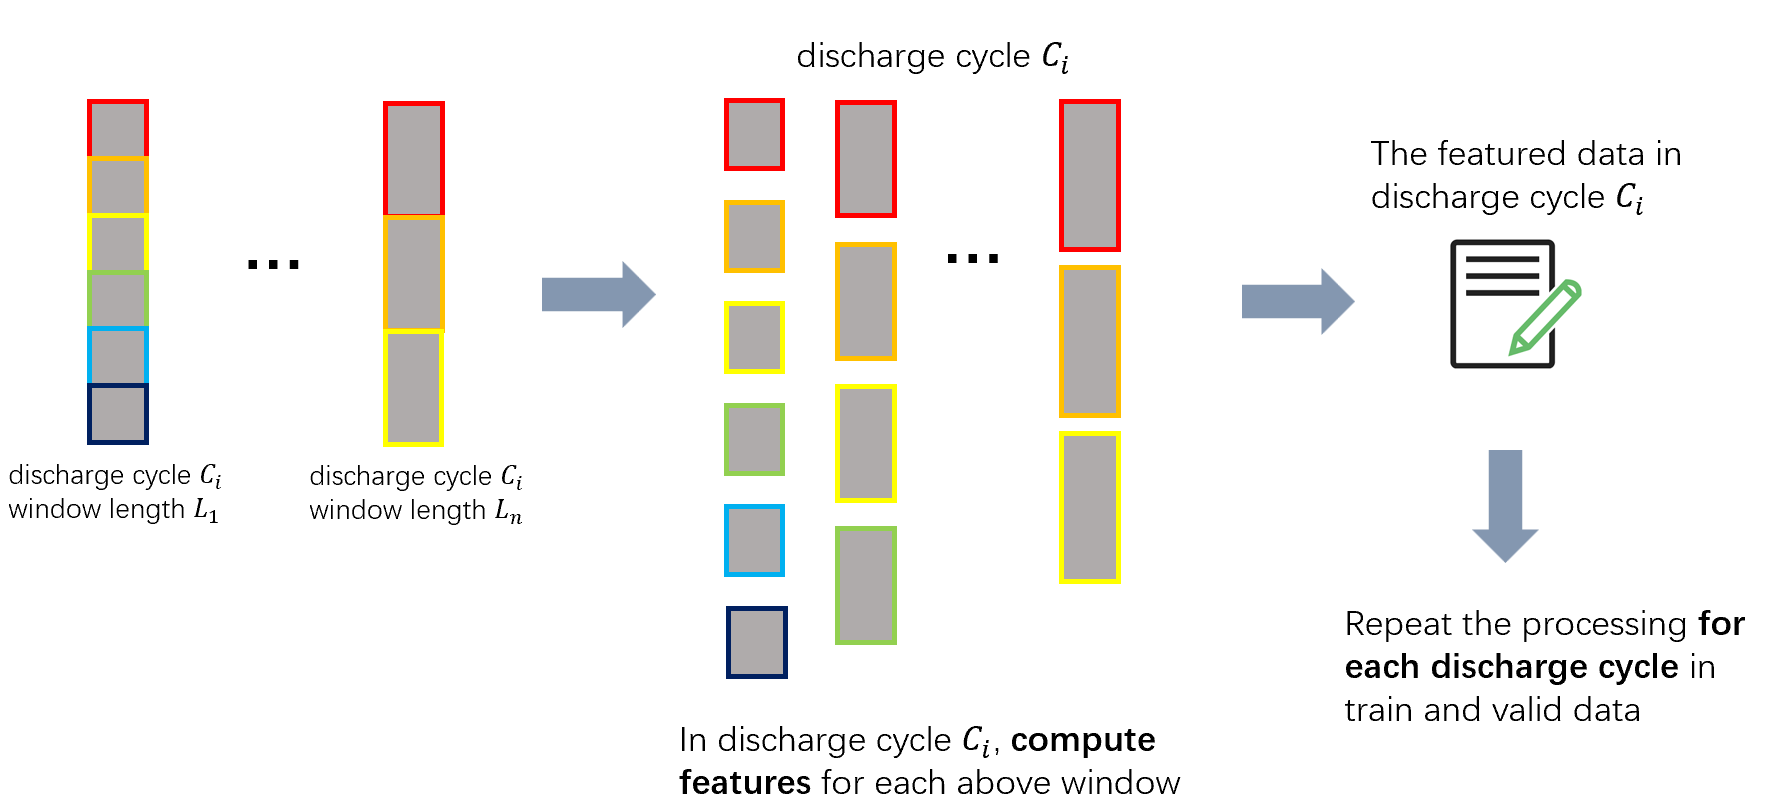
\includegraphics[width=\textwidth]{ch3_window_segmentation.png}
    \end{column}
    \begin{column}{0.40\textwidth}
      \begin{itemize}
        \item $wlen \in \{20, 30, 40, 50, 60\}$
        \item non-overlapping, stride = $wlen$
        \item label = SoH of the window's last sample
        \item $\approx\!5\times$ more training samples: the same discharge event
              at five resolutions, always the same label
      \end{itemize}
    \end{column}
  \end{columns}
  \begin{block}{Training objective}
    Regardless of window length, predict the \textbf{same} SoH.
  \end{block}
\end{frame}
\note{Instead of one fixed window length, I train on five at once. The same
physical discharge event appears at five resolutions, always with the same SoH
label. The model learns that length itself must not matter. This is the inductive
bias that pays off in the generalization experiment.}

% ---- 8. Feature extraction ----
\begin{frame}{Feature extraction: the 10-D vector}
  \begin{columns}[T]
    \begin{column}{0.42\textwidth}
      \textbf{Raw window} ($wlen \times 4$: $V, I, T, t$)\\[0.4em]
      {\small 5 intermediate signals:}\\[0.2em]
      \begin{itemize}
        \item $\dot V = dV/dt$
        \item $\dot T = dT/dt$
        \item $P = V \cdot I$
        \item $Q = \int I\,dt$
        \item $dV/dQ$ \ --- the IC-analysis quantity
      \end{itemize}
      \vspace{0.3em}
      \textbf{Key property:} the input dimension no longer depends on window length.
    \end{column}
    \begin{column}{0.52\textwidth}
      \textbf{10 features:}\\[0.3em]
      {\small
      \begin{tabular}{@{}ll@{\quad}ll@{}}
        1 & mean($dV/dt$) & 6 & mean($dV/dQ$)\\
        2 & mean($V$) & 7 & max($dV/dQ$)\\
        3 & mean($dT/dt$) & 8 & min($dV/dQ$)\\
        4 & mean($V \cdot I$) & 9 & window duration\\
        5 & mean($t_{rel}$) & 10 & mean($T$)\\
      \end{tabular}}
      \vspace{0.4em}
      \begin{itemize}
        \item physically motivated: $dV/dQ$ peak shifts track degradation
        \item the same logic hand-written in C on the MCU (FPU, float32)
      \end{itemize}
    \end{column}
  \end{columns}
\end{frame}
\note{This is the key design decision. The model never sees the raw time series,
it sees ten statistics, chosen the way a battery engineer would look at
degradation. Any window length maps to the same ten numbers, so one model serves
every length. Feature extraction is the decoupling point between the field and the
model.}

% ---- 9. From Python to MCU ----
\begin{frame}[fragile]{From Python to MCU: LightGBM $\rightarrow$ self-contained C}
  \begin{columns}[T]
    \begin{column}{0.43\textwidth}
      \begin{itemize}
        \item \textbf{Why LightGBM}: no matrix multiplications, no activations;
              inference = threshold compares + additions
        \item \textbf{Optuna} Bayesian search, 1000 trials, $max\_depth \le 8$
              (Flash budget $\sim O(N_{trees} \times 2^{depth})$)
        \item \textbf{EDEN compiler} $\rightarrow$ 4 static const arrays,
              6 bytes per node
        \item Firmware = HAL init + feature extraction + inference + main loop
        \item MCU output matches Python \textbf{bit-for-bit}
      \end{itemize}
    \end{column}
    \begin{column}{0.55\textwidth}
      {\footnotesize
      \begin{verbatim}
float output = 0;
for (int t = 0; t < N_TREES; t++) {
  int idx = roots[t];
  while (features[idx] != LEAF) {
    if (input[features[idx]] <= alphas[idx])
      idx++;                 // left
    else
      idx += children_right[idx];
  }
  output += alphas[idx];
}
return output;
      \end{verbatim}}
      No recursion, no malloc, no dependencies.
    \end{column}
  \end{columns}
\end{frame}
\note{A tree ensemble is nothing but thresholds and additions, the cheapest
operations an MCU can run. I tuned it with one thousand Bayesian trials under a
depth cap that guarantees the Flash budget. EDEN compiles the ensemble into four
const arrays; my firmware calls feature extraction, then inference. The MCU output
matches Python bit-for-bit.}

% ================================================================
%  Evaluation
% ================================================================
\section{Evaluation}

% ---- 10. Experimental setup ----
\begin{frame}{Experimental setup: two datasets, one fair baseline}
  \begin{columns}[T]
    \begin{column}{0.56\textwidth}
      {\small
      \begin{tabular}{@{}lll@{}}
        \toprule
        & \textbf{NBD} & \textbf{NRD}\\
        \midrule
        Cells & 19 & 28\\
        Discharge cycles & 164 & 258\\
        Sampling rate & 0.09 Hz & 0.33 Hz\\
        Label & capacity (Ah) & SoH (\%) \\
        Load profile & constant current & randomized 0.5--4 A\\
        \bottomrule
      \end{tabular}}
      \vspace{0.5em}
      \begin{itemize}
        \item cycle-level 64/16/20 split --- no leakage across windows
        \item NRD: cross-cell isolation enforced
      \end{itemize}
    \end{column}
    \begin{column}{0.42\textwidth}
      \begin{itemize}
        \item \textbf{BiLSTM baseline} (Sammartino et al.) reproduced:
              retrained on the \emph{same} split, deployed on the \emph{same}
              SPC58EC80E5
        \item Hardware: 180 MHz, 4 MB Flash, 384 KB SRAM
        \item Metrics: MAE / MSE, inference cycles, Flash \& RAM
      \end{itemize}
    \end{column}
  \end{columns}
\end{frame}
\note{Fairness is the point here: same datasets, same split, same silicon. The NBD
set is the baseline's own dataset; the NRD set with its randomized loads is the
harder, more realistic test.}

% ---- 11. Accuracy ----
\begin{frame}{Accuracy vs BiLSTM}
  \begin{center}
    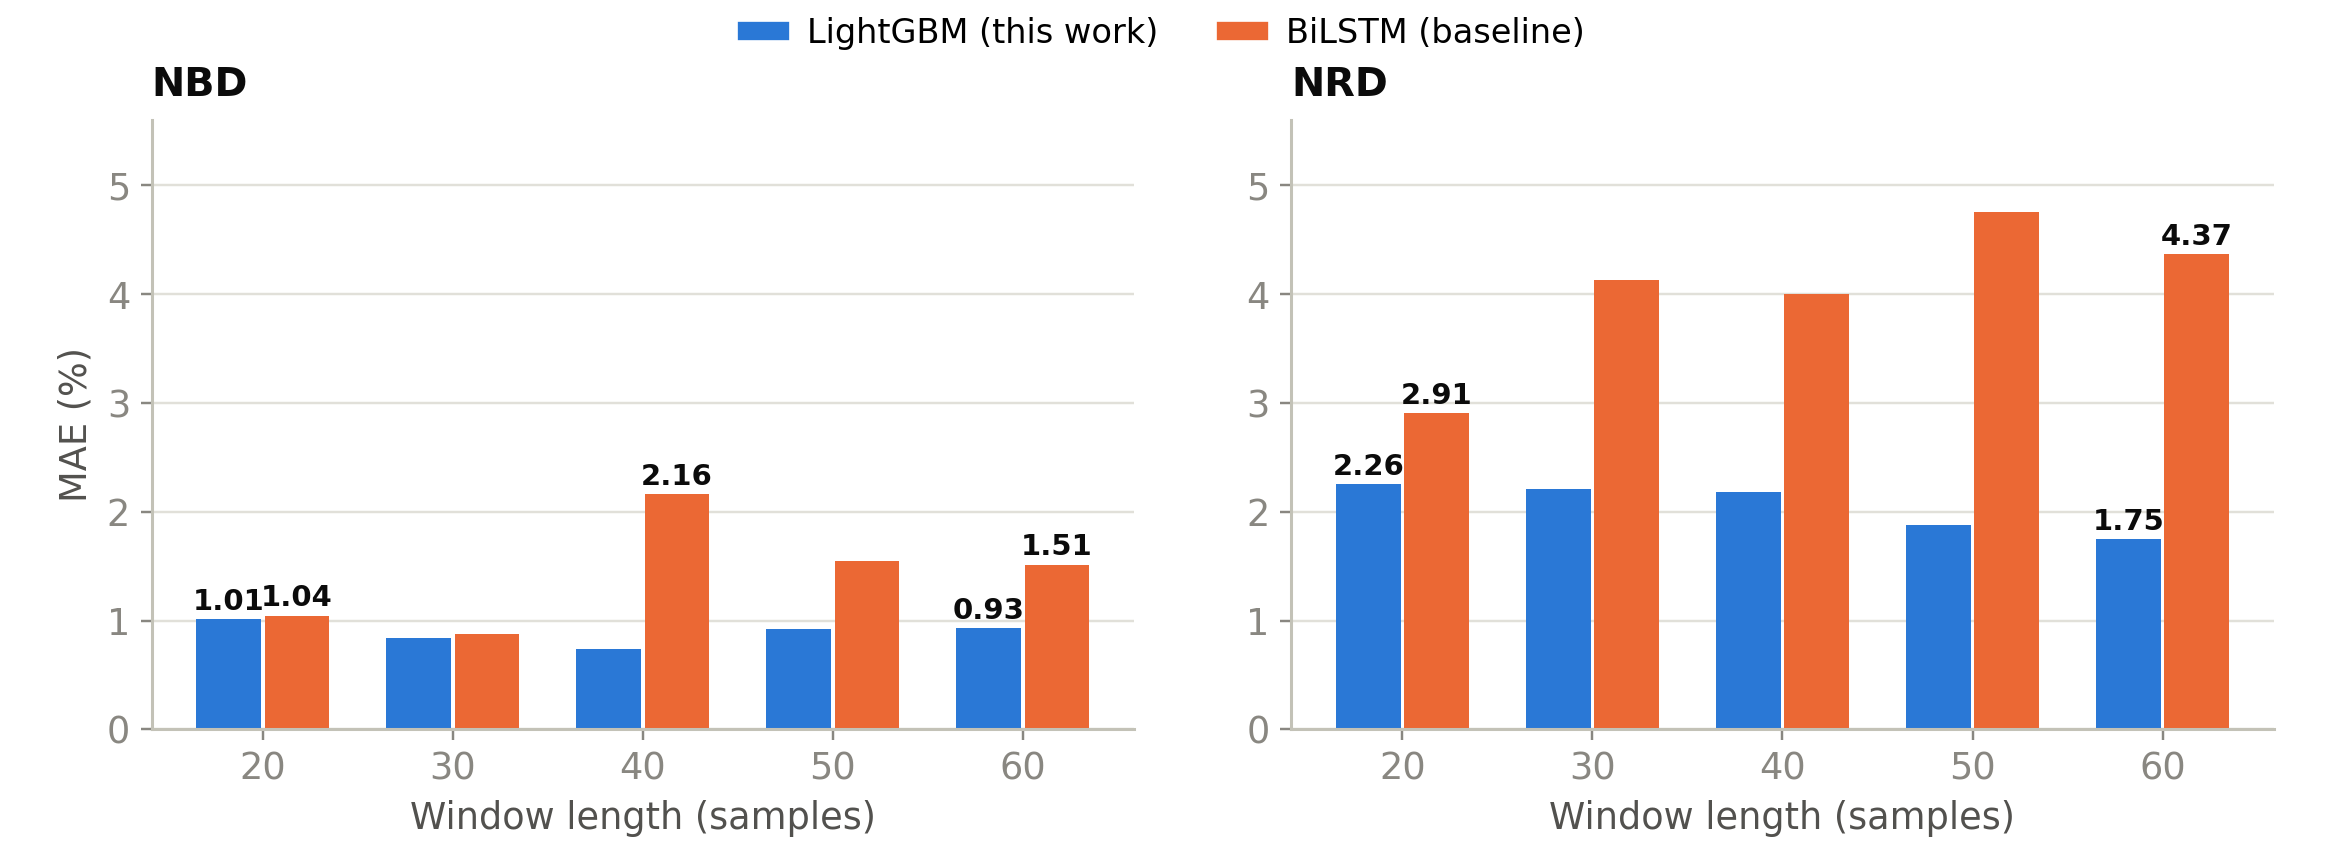
\includegraphics[width=0.92\textwidth]{fig_mae_vs_wlen.png}
  \end{center}
  \begin{block}{}
    \textbf{NBD @ $wlen$ 20}: FW MAE \textbf{0.0167} vs 0.0202 ($-17\%$) ---
    \textbf{NRD}: LightGBM 2.26 $\rightarrow$ 1.75 (longer windows help) vs
    BiLSTM 2.91 $\rightarrow$ 4.37 (longer windows hurt)
  \end{block}
\end{frame}
\note{On the baseline's own dataset we are slightly ahead. On the
randomized-usage dataset the gap is 2.5 times at the longest window, and look at
the directions: our error falls as windows lengthen, the LSTM's grows. That
direction matters because real deployments trend toward longer, higher-rate
windows.}

% ---- 12. Efficiency ----
\begin{frame}{Efficiency \& memory footprint}
  \begin{center}
    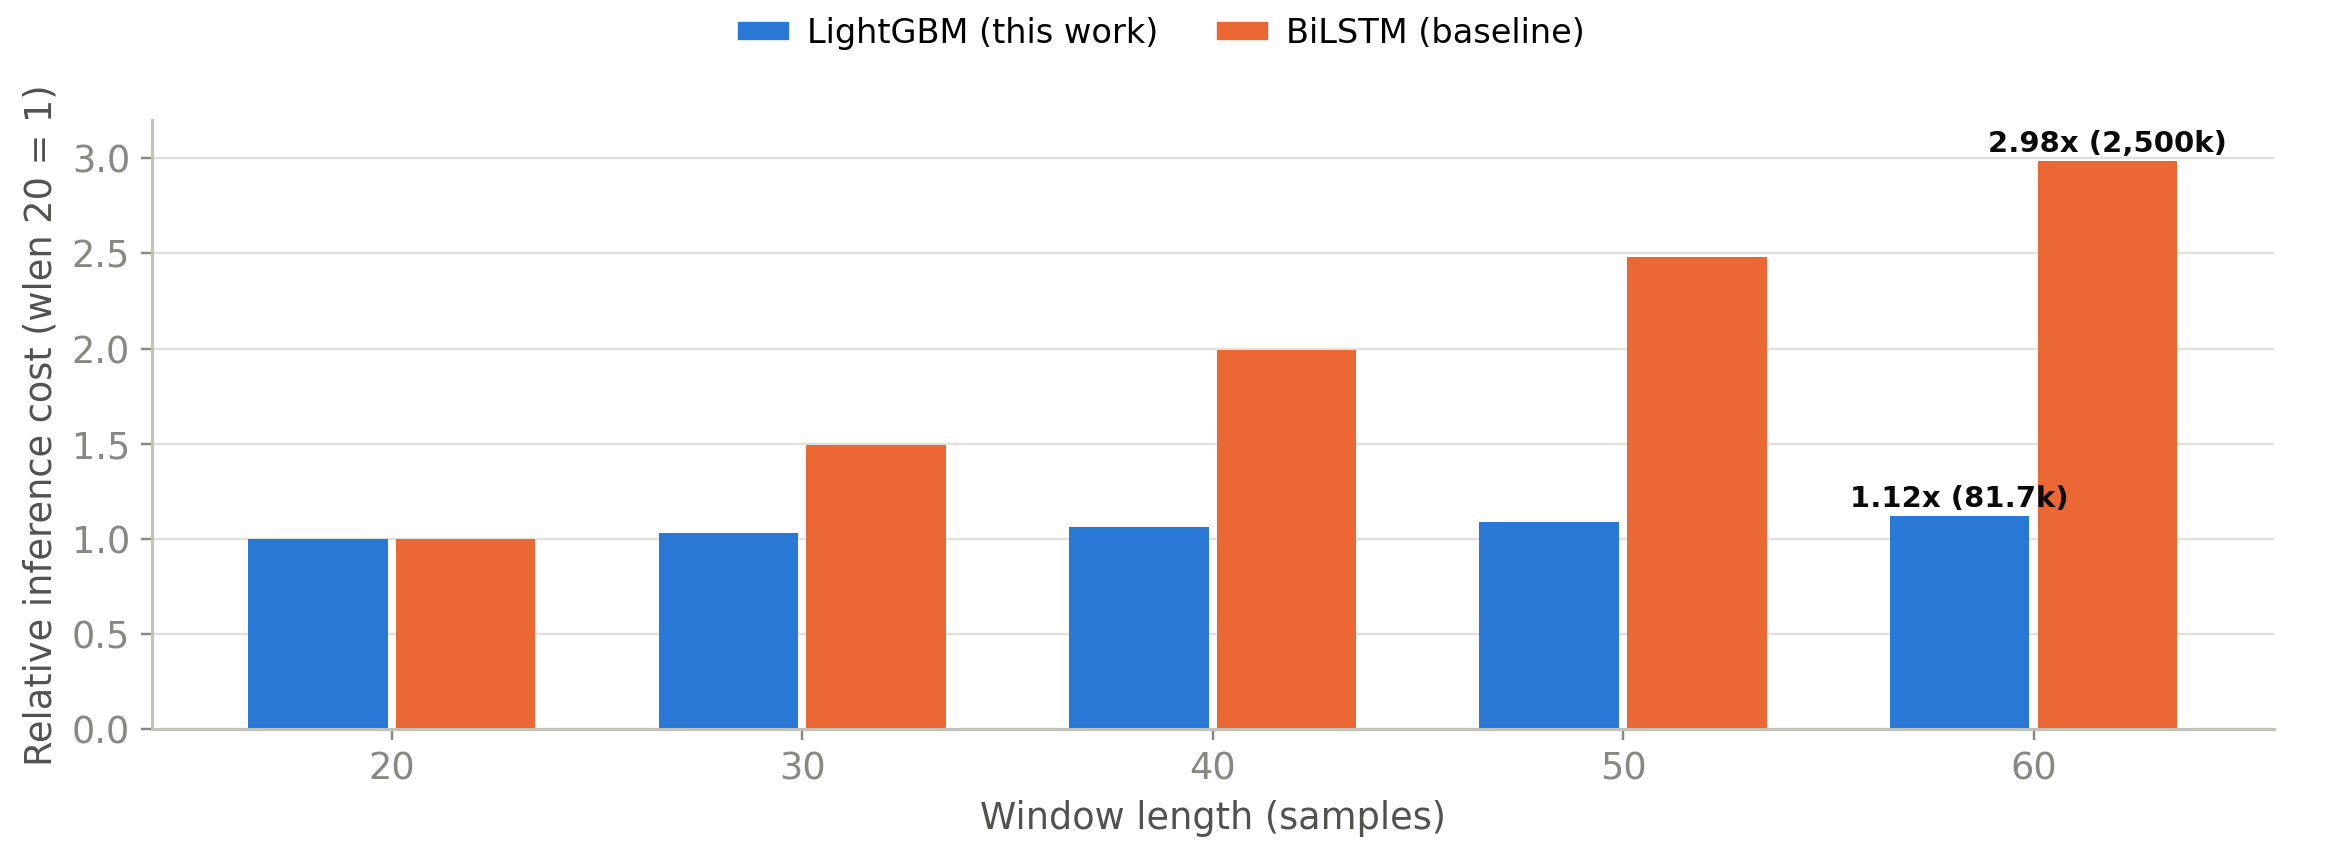
\includegraphics[width=0.92\textwidth]{fig_cycles_vs_wlen.png}
  \end{center}
  \begin{block}{}
    \textbf{11.6$\times$} faster at $wlen$ 20 (0.403 ms vs 4.656 ms) ---
    \textbf{30.7$\times$} at $wlen$ 60 ---
    Flash \textbf{$<$ 3\%} (91--111 KB) --- RAM 0.49\% (1.88 KB) ---
    energy 24 $\mu$J vs 279 $\mu$J
  \end{block}
\end{frame}
\note{The headline is 11 to 30 times faster. But the trend is the real story: our
cost is nearly flat because tree traversal is constant, only the feature loop
grows. That flatness is what keeps the BMS real-time budget safe as sampling rates
rise.}

% ---- 13. Generalization ----
\begin{frame}{Generalization to unseen window lengths}
  \begin{columns}[T]
    \begin{column}{0.52\textwidth}
      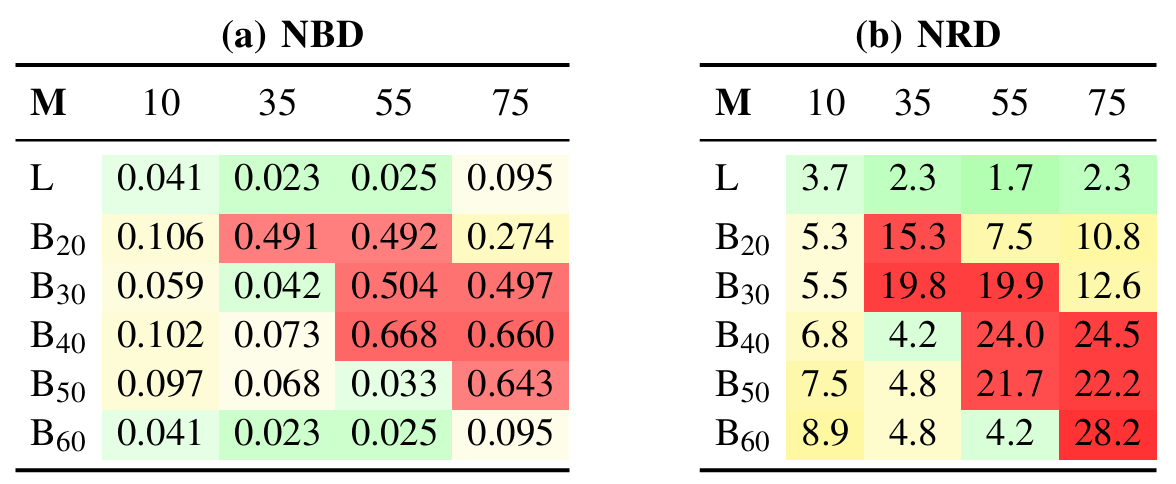
\includegraphics[width=\textwidth]{ch4_generalization.png}
    \end{column}
    \begin{column}{0.46\textwidth}
      \small
      \begin{itemize}
        \item Test lengths $\{10, 35, 55, 75\}$ --- inside and outside the training range
        \item Avg MAE, NBD: \textbf{0.046} vs 0.21--0.38 (BiLSTM variants)
        \item Avg MAE, NRD: \textbf{2.50} vs 9.7--14.9 \quad ($4$--$6\times$)
        \item Extreme case: BiLSTM$_{60}$ jumps 4.2 $\rightarrow$ \textbf{28.2}
              from length 55 to 75
      \end{itemize}
      \begin{alertblock}{Why}
        LightGBM consumes \emph{features}, not sequences --- truncation and
        zero-padding are artifacts an LSTM was never trained to see.
      \end{alertblock}
    \end{column}
  \end{columns}
\end{frame}
\note{This is the experiment that matters for deployment. A firmware update
changes the sampling rate, an unusual trip breaks the window assumption. One
LightGBM model, without any modification, stays accurate. Every BiLSTM variant
collapses somewhere, by up to 7 times between two lengths 15 samples apart.}

% ================================================================
%  OTA design
% ================================================================
\section{OTA Design}

% ---- 14. OTA ----
\begin{frame}{OTA update architecture --- closing the Digital Twin loop}
  \begin{columns}[T]
    \begin{column}{0.42\textwidth}
      \textbf{Role}\\[0.2em]
      The SoC model consumes the SoH estimate $\Rightarrow$ it must be
      refreshed as the battery ages.\\[0.6em]
      \textbf{Triggers}\\[0.2em]
      \begin{itemize}
        \item SoH drift $> 1$ pt since last update
        \item or 6-month timeout (safety net)
      \end{itemize}
      \vspace{0.4em}
      \textbf{Security \& recovery}\\[0.2em]
      {\small SHA-256 + signature \ $\cdot$ \ monotonic version numbers\\
      A/B rollback \ $\cdot$ \ cloud alerting}
    \end{column}
    \begin{column}{0.56\textwidth}
      \textbf{Update lifecycle (8 steps)}
      \begin{enumerate}
        \item on-board data accumulation
        \item periodic upload (safe state, TCU)
        \item trigger evaluation
        \item cloud retraining of the SoC model
        \item validation + packaging + signing
        \item OTA delivery (hash + signature check)
        \item A/B partition installation
        \item model switch + confirmation
      \end{enumerate}
    \end{column}
  \end{columns}
  \vspace{0.5em}
  \alert{Architectural design --- not implemented in hardware (future work).}
\end{frame}
\note{Because the SoC model consumes the SoH estimate, it must be refreshed as the
battery ages; that is what OTA is for. I designed the complete lifecycle, from
on-board data accumulation to A/B partition switch, with signatures and rollback.
To be clear: this is a design, and its implementation is the first item of future
work.}

% ================================================================
%  Conclusions
% ================================================================
\section{Conclusions}

% ---- 15. Conclusions ----
\begin{frame}{Conclusions}
  \begin{enumerate}
    \item \textbf{Accuracy} --- matches or beats BiLSTM on both datasets
    \item \textbf{Efficiency} --- 11--30$\times$ faster; $<$ 3\% Flash, 0.49\% RAM
    \item \textbf{Robustness} --- one model, unseen window lengths, no retraining
  \end{enumerate}
  \vspace{0.5em}
  \begin{block}{}
    SoH is the foundation of the dual-model Digital Twin --- and the foundation
    now exists: \textbf{trained, compiled, deployed, and measured on real
    automotive silicon}.
  \end{block}
\end{frame}
\note{Back to where I started: SoH is the foundation of the digital twin, and the
foundation now exists, trained, compiled, deployed, and measured on real
automotive silicon.}

% ---- 16. Future work ----
\begin{frame}{Future work}
  \begin{itemize}
    \item Implement the OTA mechanism on hardware (end-to-end validation)
    \item Integrate the SoC model --- handle SoH-to-SoC error propagation
          (e.g.\ inject synthetic SoH noise during training)
    \item Validate on real-world vehicle data
    \item Model quantization (16/8-bit)
    \item Federated, privacy-preserving training
  \end{itemize}
\end{frame}
\note{Each of these is a direction I can discuss in the questions.}

% ---- 17. Thanks ----
\begin{frame}[plain]
  \begin{center}
    {\Large\bfseries Thank you --- Questions?}\\[1.2em]
    Code \& pipeline: \url{https://github.com/QYRR/batteryML}
  \end{center}
\end{frame}

% ================================================================
%  Backup slides
% ================================================================
\appendix
\section*{Backup}

% ---- B1: methods matrix ----
\begin{frame}{Backup: why LightGBM? --- method comparison}
  {\small
  \begin{tabular}{@{}lccccc@{}}
    \toprule
    Method & Accuracy & Cost & \makecell[l]{MCU-\\deployable} & \makecell[l]{Input\\flexibility}\\
    \midrule
    Electrochemical & Very high & Very high & No & ---\\
    ECM + Filter & Moderate & Low & Yes & ---\\
    Classical ML & Moderate--High & Moderate & Limited & Yes\\
    Deep Learning & High & High & Limited & No\\
    LightGBM & High & Very low & Yes & Yes\\
    \bottomrule
  \end{tabular}}
  \vspace{0.5em}
  \begin{itemize}
    \item LightGBM is the only row combining high accuracy with freedom from
          fixed-length inputs (through feature extraction)
  \end{itemize}
\end{frame}

% ---- B2: raw data ----
\begin{frame}{Backup: raw data structure}
  \begin{center}
    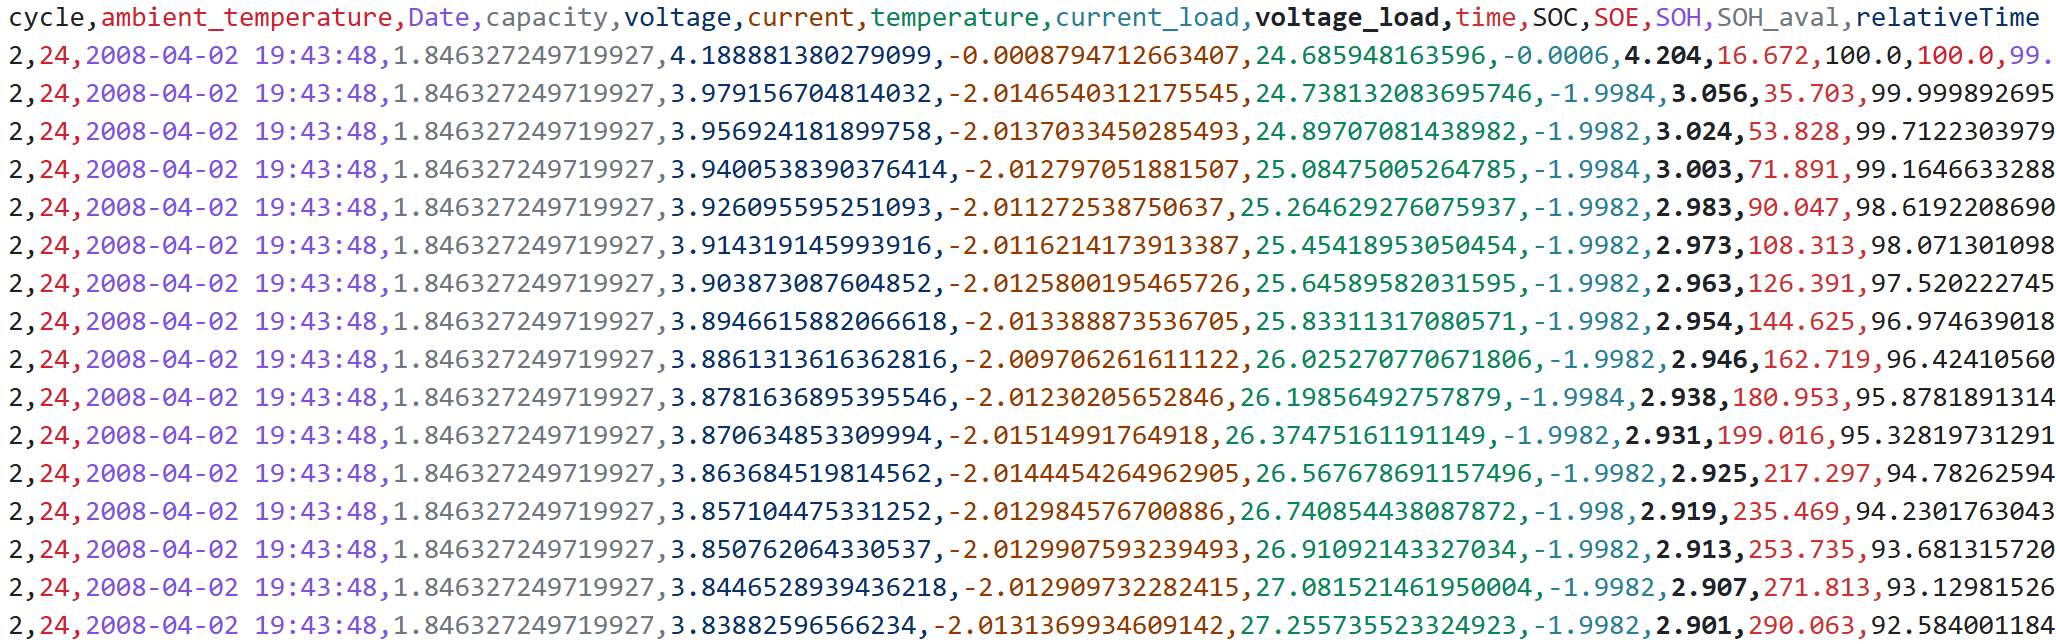
\includegraphics[width=0.82\textwidth]{ch3_inputdata_sample.png}
  \end{center}
  {\small Rows are sampling instants within a discharge cycle; every row of a
  cycle shares the same SoH label.}
\end{frame}

% ---- B3: deployment table ----
\begin{frame}{Backup: full deployment results (Table 4.4)}
  {\scriptsize
  \begin{columns}[T]
    \begin{column}{0.5\textwidth}
      \centering\textbf{NBD}\\[0.2em]
      \begin{tabular}{@{}rcccccc@{}}
        \toprule
        WL & M & MAE\% & MSE\%$^2$ & kcyc & RAM\% & Flash\%\\
        \midrule
        20 & L & 1.013 & 2.321 & 72.6 & 0.49 & 2.71\\
        20 & B & 1.045 & 2.031 & 838 & 0.13 & 0.21\\
        30 & L & 0.840 & 1.741 & 74.7 & 0.49 & 2.71\\
        30 & B & 0.873 & 1.451 & 1250 & 0.13 & 0.21\\
        40 & L & 0.738 & 1.161 & 77.1 & 0.49 & 2.71\\
        40 & B & 2.160 & 7.544 & 1670 & 0.13 & 0.21\\
        50 & L & 0.921 & 2.321 & 79.0 & 0.49 & 2.71\\
        50 & B & 1.551 & 4.062 & 2080 & 0.13 & 0.21\\
        60 & L & 0.932 & 1.741 & 81.3 & 0.49 & 2.71\\
        60 & B & 1.514 & 3.772 & 2500 & 0.13 & 0.21\\
        \bottomrule
      \end{tabular}
    \end{column}
    \begin{column}{0.5\textwidth}
      \centering\textbf{NRD}\\[0.2em]
      \begin{tabular}{@{}rcccccc@{}}
        \toprule
        WL & M & MAE\% & MSE\%$^2$ & kcyc & RAM\% & Flash\%\\
        \midrule
        20 & L & 2.256 & 12.622 & 73.3 & 0.49 & 2.23\\
        20 & B & 2.908 & 14.897 & 838 & 0.13 & 0.21\\
        30 & L & 2.208 & 11.788 & 75.4 & 0.49 & 2.23\\
        30 & B & 4.127 & 27.588 & 1250 & 0.13 & 0.21\\
        40 & L & 2.183 & 10.498 & 77.8 & 0.49 & 2.23\\
        40 & B & 4.002 & 28.180 & 1670 & 0.13 & 0.21\\
        50 & L & 1.881 & 7.137 & 79.6 & 0.49 & 2.23\\
        50 & B & 4.751 & 40.870 & 2080 & 0.13 & 0.21\\
        60 & L & 1.751 & 7.357 & 82.0 & 0.49 & 2.23\\
        60 & B & 4.368 & 30.323 & 2500 & 0.13 & 0.21\\
        \bottomrule
      \end{tabular}
    \end{column}
  \end{columns}}
  {\scriptsize L = LightGBM (this work), B = BiLSTM. MAE/MSE on the SoH scale.}
\end{frame}

% ---- B4: generalization tables ----
\begin{frame}{Backup: generalization detail}
  {\scriptsize
  \begin{columns}[T]
    \begin{column}{0.5\textwidth}
      \centering\textbf{NBD --- MAE}\\[0.2em]
      \begin{tabular}{@{}lcccc c@{}}
        \toprule
        Model & 10 & 35 & 55 & 75 & Avg\\
        \midrule
        LightGBM & 0.041 & 0.023 & 0.025 & 0.095 & 0.046\\
        BiLSTM$_{20}$ & 0.106 & 0.491 & 0.492 & 0.274 & 0.341\\
        BiLSTM$_{30}$ & 0.059 & 0.042 & 0.504 & 0.497 & 0.276\\
        BiLSTM$_{40}$ & 0.102 & 0.073 & 0.668 & 0.660 & 0.376\\
        BiLSTM$_{50}$ & 0.097 & 0.068 & 0.033 & 0.643 & 0.210\\
        BiLSTM$_{60}$ & 0.041 & 0.023 & 0.025 & 0.095 & 0.046\\
        \bottomrule
      \end{tabular}
    \end{column}
    \begin{column}{0.5\textwidth}
      \centering\textbf{NRD --- MAE}\\[0.2em]
      \begin{tabular}{@{}lcccc c@{}}
        \toprule
        Model & 10 & 35 & 55 & 75 & Avg\\
        \midrule
        LightGBM & 3.7 & 2.3 & 1.7 & 2.3 & 2.50\\
        BiLSTM$_{20}$ & 5.3 & 15.3 & 7.5 & 10.8 & 9.73\\
        BiLSTM$_{30}$ & 5.5 & 19.8 & 19.9 & 12.6 & 14.45\\
        BiLSTM$_{40}$ & 6.8 & 4.2 & 24.0 & 24.5 & 14.88\\
        BiLSTM$_{50}$ & 7.5 & 4.8 & 21.7 & 22.2 & 14.05\\
        BiLSTM$_{60}$ & 8.9 & 4.8 & 4.2 & 28.2 & 11.53\\
        \bottomrule
      \end{tabular}
    \end{column}
  \end{columns}}
  {\scriptsize TODO: the NBD BiLSTM$_{60}$ row is identical to LightGBM in the
  thesis --- verify against training logs before the defense.}
\end{frame}

% ---- B5: hyperparameters ----
\begin{frame}{Backup: hyperparameter search}
  {\small
  \begin{columns}[T]
    \begin{column}{0.45\textwidth}
      \textbf{Search space}\\[0.2em]
      \begin{tabular}{@{}ll@{}}
        \toprule
        Parameter & Range\\
        \midrule
        Learning rate & $[10^{-5}, 0.7]$\\
        Max depth & $[3, 8]$\\
        Num leaves & $[2, 25]$\\
        Num estimators & $[50, 450]$\\
        $\alpha$ (L1) & $[10^{-6}, 1]$\\
        $\beta$ (L2) & $[10^{-6}, 1]$\\
        Min child samples & $[2, 25]$\\
        Column samples/tree & $[0.1, 1]$\\
        \bottomrule
      \end{tabular}
    \end{column}
    \begin{column}{0.5\textwidth}
      \textbf{Best configurations}\\[0.2em]
      \begin{tabular}{@{}lll@{}}
        \toprule
        & NBD & NRD\\
        \midrule
        LR & 0.147 & 0.085\\
        Depth & 8 & 8\\
        Leaves & 25 & 18\\
        Trees & 384 & 443\\
        $\alpha$ & $6.5\times10^{-2}$ & $1.9\times10^{-6}$\\
        $\beta$ & $6.7\times10^{-5}$ & $3.6\times10^{-4}$\\
        MCS & 6 & 17\\
        CST & 0.46 & 0.61\\
        \bottomrule
      \end{tabular}
    \end{column}
  \end{columns}}
\end{frame}

% ---- B6: EDEN representation ----
\begin{frame}[fragile]{Backup: EDEN in-memory representation}
  \begin{itemize}
    \item 4 static arrays per ensemble:
    \begin{itemize}
      \item \texttt{ROOTS} (uint16) --- start of each tree
      \item \texttt{FEATURES} (uint8) --- feature index, or leaf sentinel
      \item \texttt{ALPHAS} (float) --- split threshold, or leaf contribution
      \item \texttt{CHILDREN\_RIGHT} (uint8) --- pre-order layout: left child is implicit
    \end{itemize}
    \item 6 bytes per node --- model: 111 KB (NBD) / 91.34 KB (NRD) of 4 MB Flash
  \end{itemize}
\end{frame}

% ---- B7: OTA details ----
\begin{frame}{Backup: OTA details}
  \begin{itemize}
    \item \textbf{Update triggers}: SoH drift $>$ 1 pt \emph{or} 6-month timeout ---
          update frequency on the order of months
    \item \textbf{Delivery}: parked + sufficient battery + good signal ---
          integrity (SHA-256) and authenticity (signature) checked before install
    \item \textbf{Recovery}: anomalous outputs (SoC outside [0,100]\%, physics
          violations, deviation from Coulomb counting) $\Rightarrow$ atomic switch
          back to the previous model + cloud alert
    \item \textbf{Model OTA vs firmware OTA}: payload $\sim$100--300 KB; low risk
          --- degradation is gradual and reversible; rollback is a pointer swap
  \end{itemize}
\end{frame}

% ---- B8: SoC preliminary ----
\begin{frame}{Backup: preliminary SoC experiments}
  \begin{itemize}
    \item An SoC model with the SoH estimate as an input feature was trained and
          evaluated
    \item Finding: SoH estimation errors \textbf{propagate} into SoC predictions,
          amplifying the overall error
    \item Consequence: SoH accuracy must be established \emph{first} --- the
          dual-model cascade cannot function without a solid foundation
    \item This is why the thesis concentrates on the SoH layer
  \end{itemize}
\end{frame}

\end{document}
